

\chapter{Hematite Film Reactivity on Polycrystalline Substrates}
\label{ch:polycrystalline.reactivity}


\chintro{This chapter reports on the photochemical activity of the hematite films
supported on polycrystalline \ce{SrTiO3} substrates.\footnote{Originally, films on 
polycrystalline \ce{BaTiO3} substrates were examined. After discussions with the thesis 
committee, work on polycrystalline substrates was repeated on \ce{SrTiO3} substrates. The 
original results for films on \ce{BaTiO3} substrates are presented in the appendix to this 
document.} The area examined for reactivity
experiments was the same area used to determine the orientation relationships, discussed
later in \chapterref{polycrystalline.growth}. After reaction with the silver nitrate
solution, the reactivity of film grains was correlated to substrate and film reactivity.
The films on polycrystalline substrates present a much wider array of orientation
conditions when compared to films on single crystal substrates. This allows for the study
of the interaction between film orientation and the substrate effects observed in 
\chapterref{single.crystal.growth}.}


\section{Experimental Details}
\label{sec:poly.reac.experimental}


The photochemical activity of \ce{Fe2O3} films grown on polycrystalline \ce{SrTiO3}
substrates is reported in this chapter. An analysis of film growth and orientation
relationships is reported later in \chapterref{polycrystalline.growth}. Details on film
growth can be found in \sectionpageref{sec:poly.growth.experimental}. Electron backscatter
diffraction (\abbr{EBSD}) data from \figureref{subfilmmaps} was used to correlate
reactivity with orientation. Details for data collection can be found in
\sectionpageref{sec:poly.growth.experimental}. Before the removal of the film to analyze
substrate grain orientations, the photochemical marker reaction was performed on the film
and analyzed using optical and atomic force microscopy (\abbr{AFM}). Marker reactions were
performed as described in \sectionpageref{subsec:exp.markerreactions}. The light source
was a blue \abbr{LED}, and the reaction time was one minute. This time was selected after
trials with reaction times, and was found to result in some grains that were bare, while
other grains were highly reactive. Longer reaction times resulted in the entire surface
covered in reaction product. After these longer reaction times, silver colored material
visibly coated the reaction surface, without the aid of microscope analysis. Because the
light source was the \abbr{LED}, only visible light was available to excite electrons to
the conduction band. Because the band gap of \ce{SrTiO3} requires ultraviolet light to
generate charge carriers, all photochemical activity was attributed to the film. It was
assumed that a negligible number of charge carriers were generated in the substrate.

\section{Results}
\label{sec:poly.reac.results}

After reaction with the silver nitrate solution, the film was examined using optical and
atomic force microscopy. Optical microscopy provided a rapid, high throughput
classification of the entire area. \abbr{AFM} then confirmed the interpretation of the
optical micrograph, and provided a detailed look at small subsections of the examined
area.


\subsection{Optical Microscopy}
\label{subsec:poly.reac.optical}


\figureref{filmoptical} shows an optical micrograph of an area of the sample surface after
reaction. Dark areas on the micrograph generally indicate areas with a large amount of
reaction product. Pores are also responsible for some areas of dark contrast. Any pores
could be identified by comparison with an image of the clean sample surface. The image of
the clean surface also served as a reference, verifying that dark contrast was not
present. The clean surface is uniformly bright, with the exception of pores, cracks, and
grain boundaries. These areas appear as dark spots on the micrograph. Some grains appear
slightly darker than others. This is a result of differing interaction with the polarized
light, and does not represent reaction product on the surface. \figureref{filmclean} shows
the surface after reaction product was cleaned, for comparison with the image in
\figureref{filmoptical}.
\begin{figure}
\begin{center}
	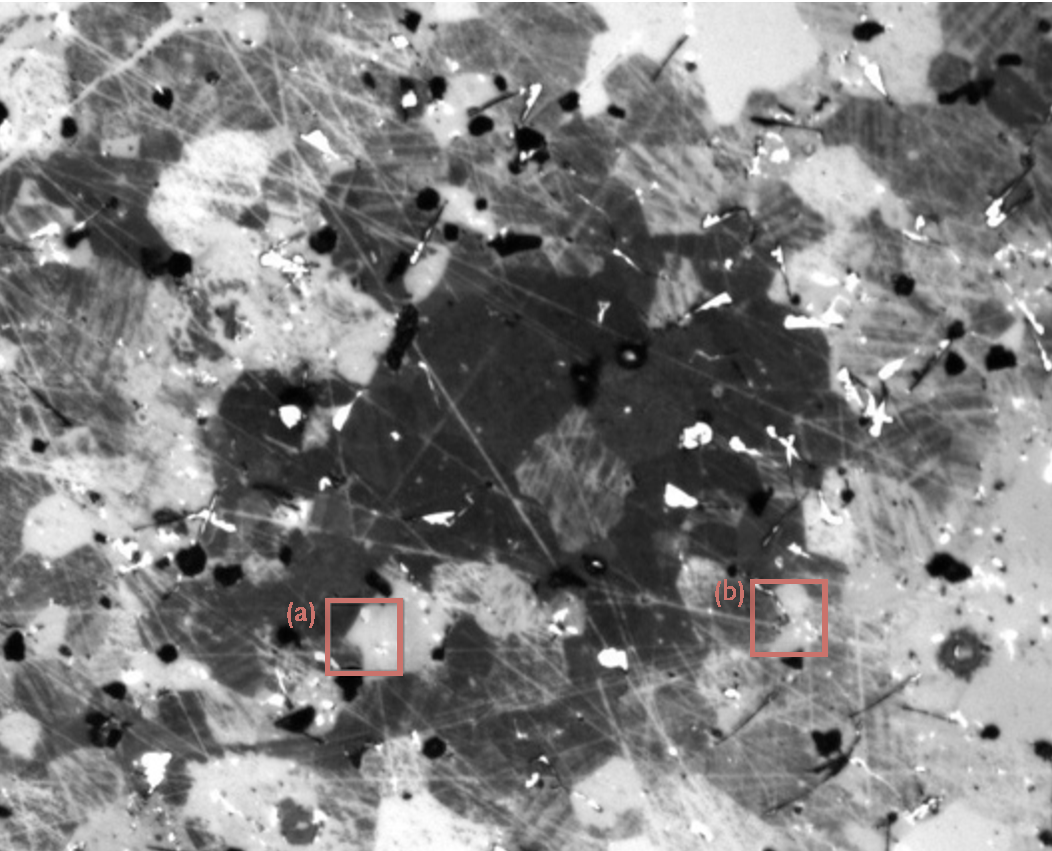
\includegraphics[width=0.8\textwidth]{filmoptical.pdf}
		\caption[Film surface after reaction]{%
			Surface of \ce{Fe2O3} film on polycrystalline
			\ce{SrTiO3} substrate after marker reaction. Areas
			of dark contrast correspond to portions of the surface
			covered with a large amount of reaction product.
			Bright areas are bare areas, with little reaction
			product. The outlined boxes correspond to the areas
			presented in the \abbr{AFM} micrographs in Figure~\ref{fig:filmafm}. }
	\label{fig:filmoptical}
	\end{center} 
\end{figure}
%
%
\begin{figure}
\begin{center}
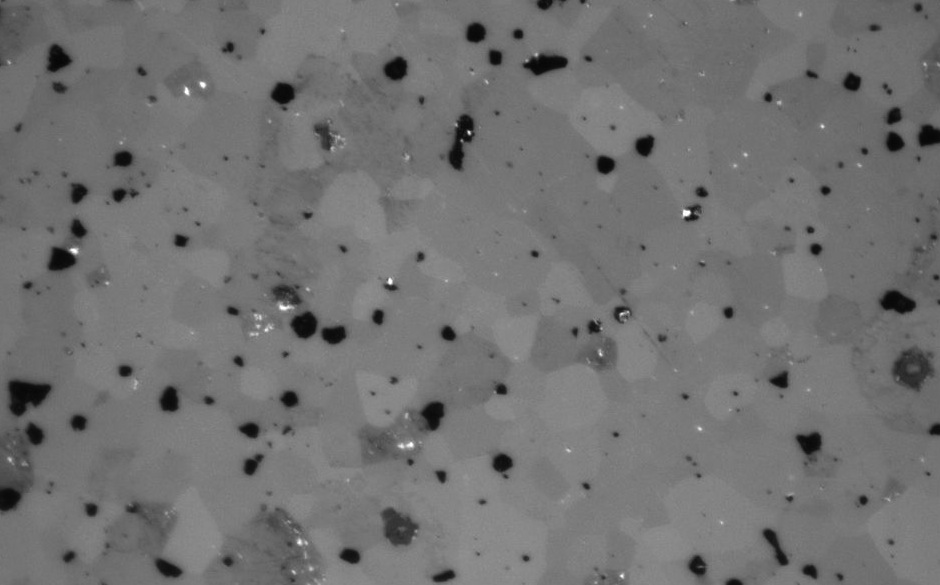
\includegraphics[width=0.8\textwidth]{filmclean.jpg}
\caption[Cleaned film surface]{%
	Surface of \ce{Fe2O3} film on polycrystalline \ce{SrTiO3} 
	substrate after cleaning. The surface shows uniform contrast, exception pores, cracks,
and the affect of light polarization,
	supporting the interpretation of contrast in \figureref{filmoptical}.}
\label{fig:filmclean}
\end{center}
\end{figure}
%\sidefigure[Cleaned film surface.]{%
%	Surface of \ce{Fe2O3} film on polycrystalline \ce{SrTiO3} 
%	substrate after cleaning. The surface shows uniform contrast,
%	supporting the interpretation of contrast in \figureref{filmoptical}.
%	\label{fig:filmclean}
%	}{%
%	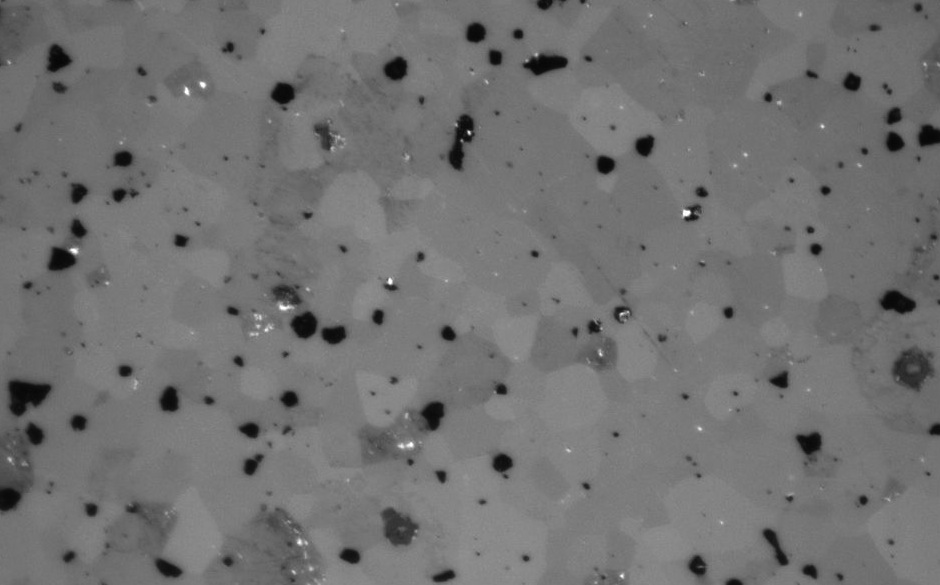
\includegraphics[width=\marginparwidth]{filmclean.jpg}
%}{0} % Last argument is number of lines to move up or down

Using the electron backscatter diffraction maps in \figureref{subfilmmaps} as a guide,
each individual film grain was identified in the optical image in \figureref{filmoptical}.
The identified grains were manually classified as highly reactive, moderately reactive, or
nonreactive. Grains that were uniformly dark were classified as highly reactive.
Conversely, grains that were uniformly bright were nonreactive. Grains that appeared a
medium gray color, or were otherwise not uniformly covered by reaction product were
labelled moderately reactive.

\figureref{labeledgrains} shows a digram of the resulting classifications. The grain
boundaries were taken from the \abbr{EBSD} map of the substrate. Dark blue portions of
this map correspond to highly reactive grains, medium blue to moderately reactive grains,
and light blue areas are nonreactive grains. White corresponds to areas where no
assignment was made. This occurred when it was unclear the reactivity level of a grain,
owing to image artifacts or difficulty distinguishing grains. Also, some white grains in
\figureref{labeledgrains} were outside the field of view of the microscope image in
\figureref{filmclean}.
\begin{figure}
	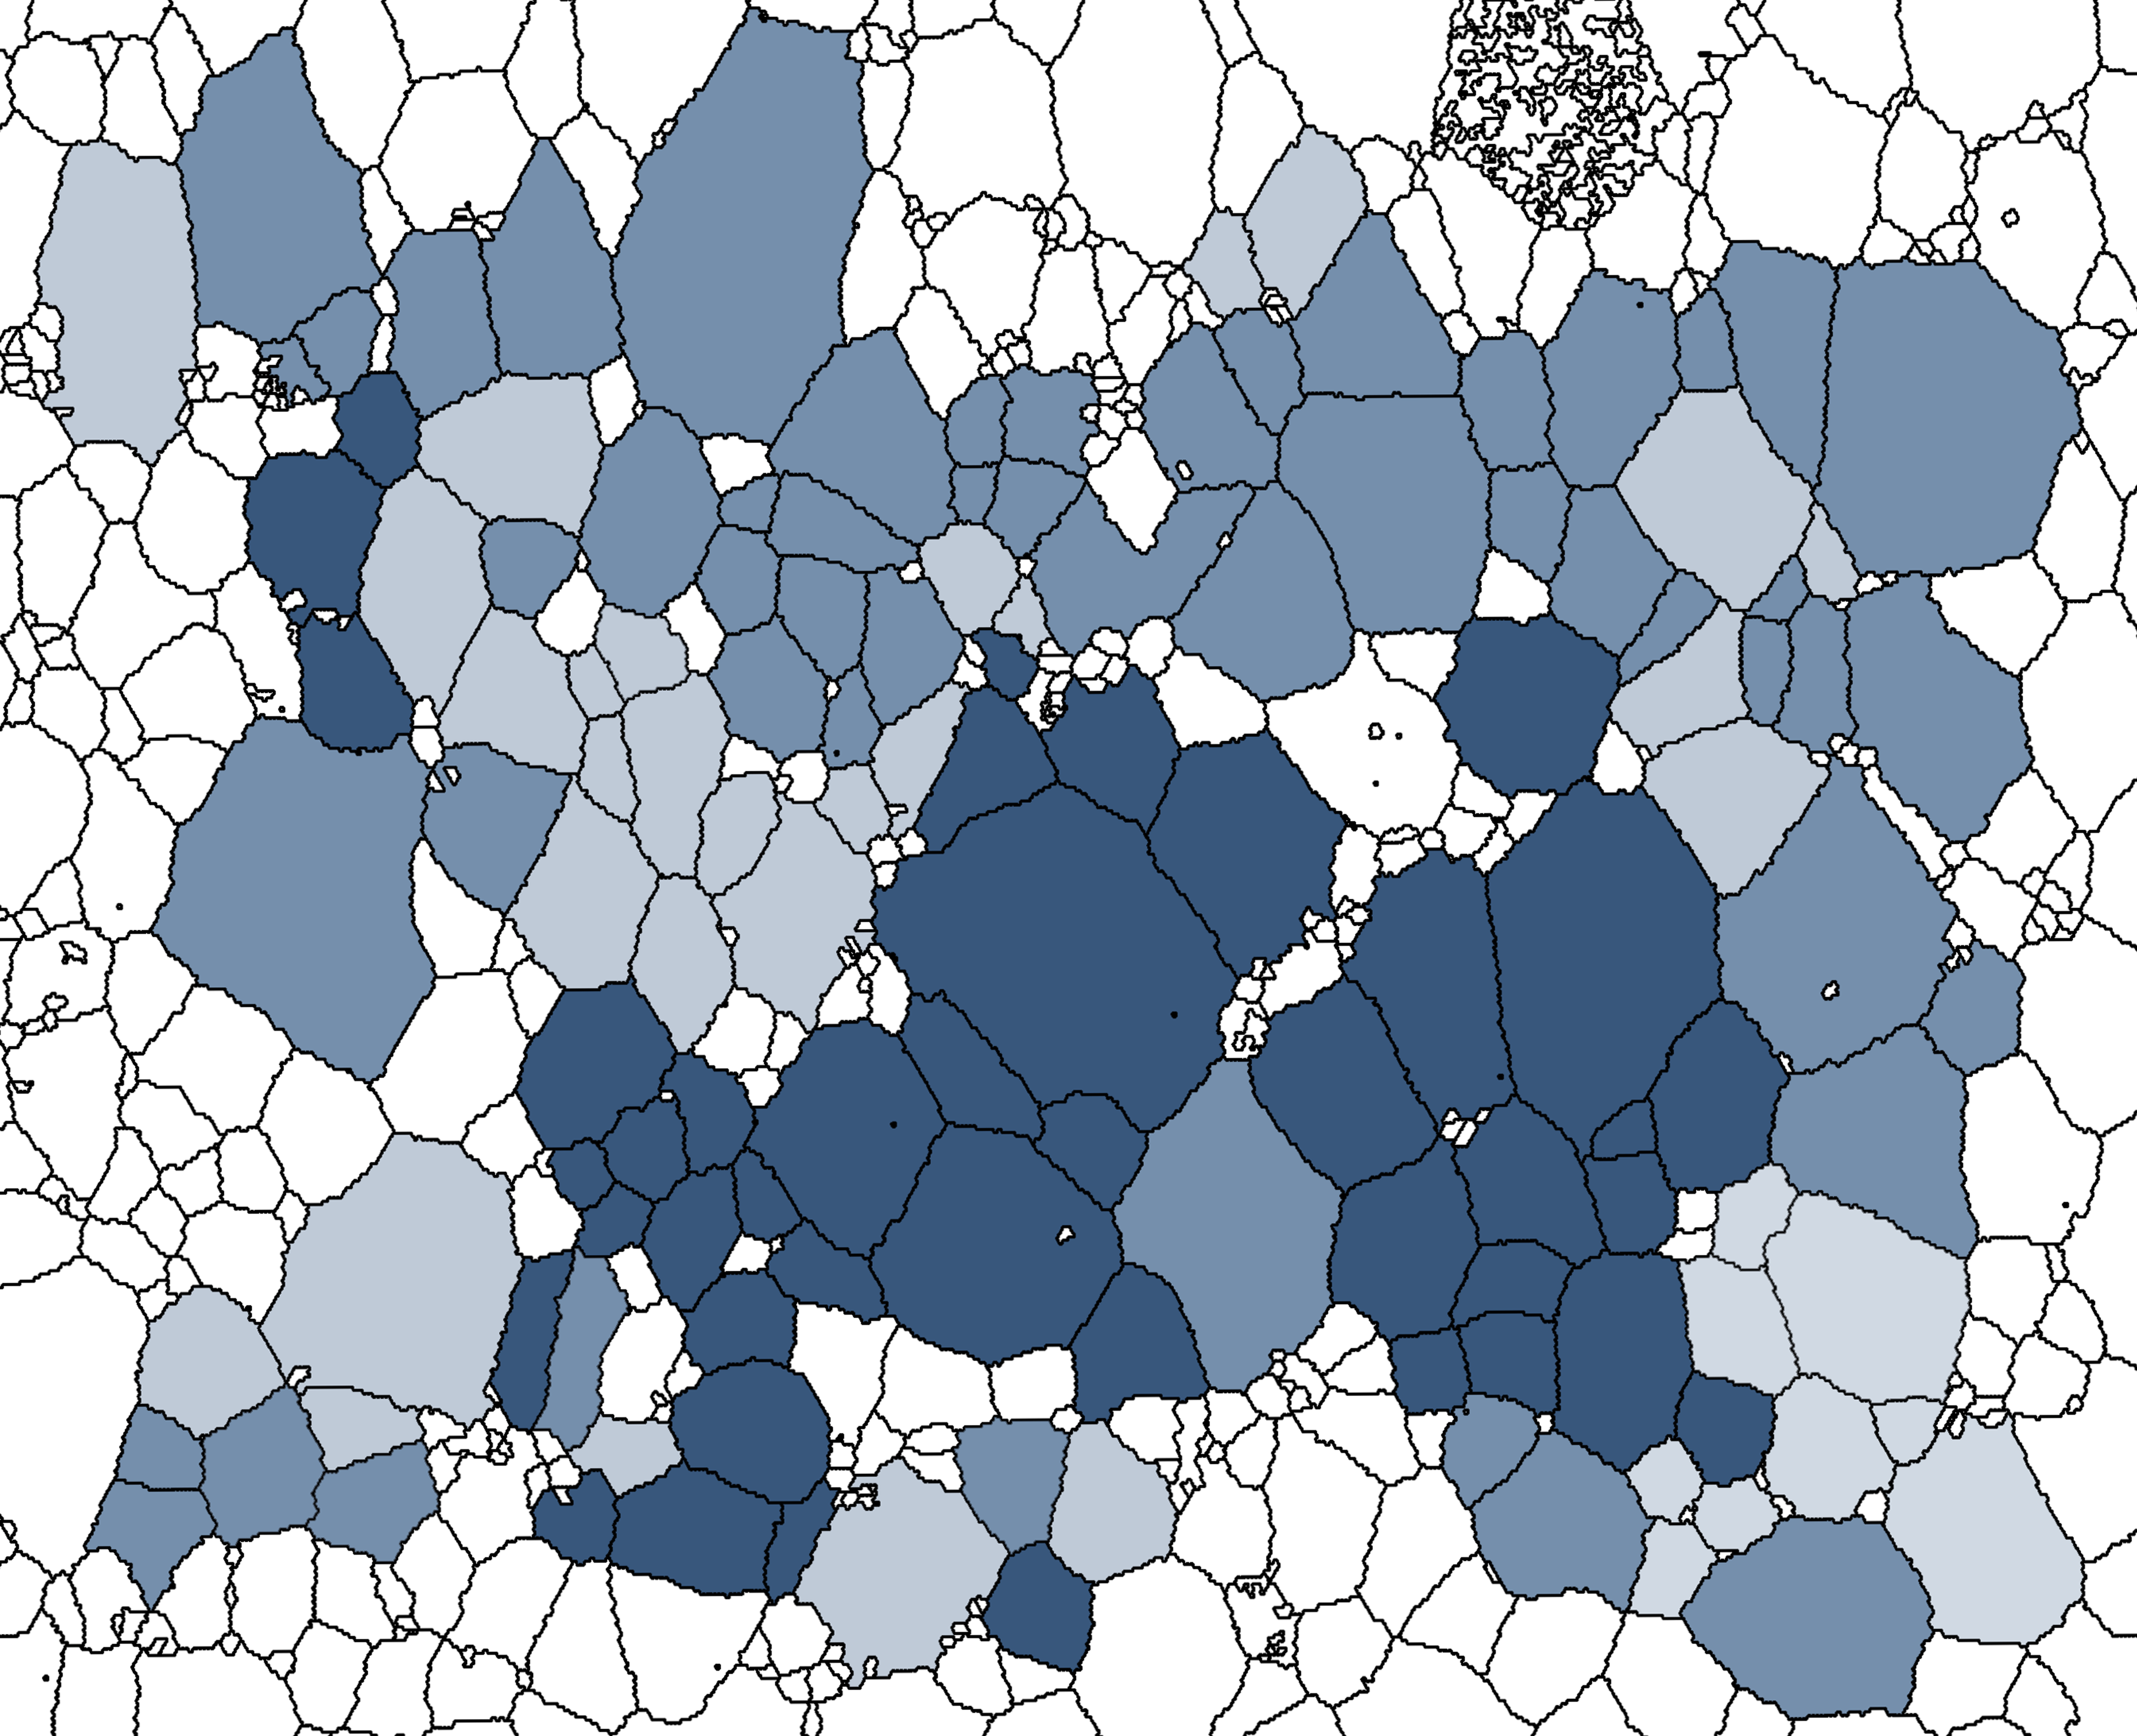
\includegraphics[width=\textwidth]{labeledgrains.pdf}
		\caption[Reactivity assignments for film]{%
			Grain boundary network taken from \abbr{EBSD} data in 
			\figureref{subfilmmaps}(b) with assignments of reactivity
			observed in \figureref{filmclean}. Dark blue represents 
			highly reactive grains, medium blue represents moderately
			reactive grains, and light blue represents nonreactive 
			grains. White grains are those that were not assigned a 
			reactivity level.}
	\label{fig:labeledgrains}
\end{figure}

The orientation of the substrate and film grains was plotted on the standard stereographic
triangles for cubic and hexagonal crystal structures respectively. These plots are
depicted in \figureref{substrateplot} and \ref{fig:filmplots}. Both film and substrate
orientations were examined to determine whether any reactivity differences were a result
of substrate or film orientation alone, or a combination of the two.

\begin{figure}
	\begin{center}
	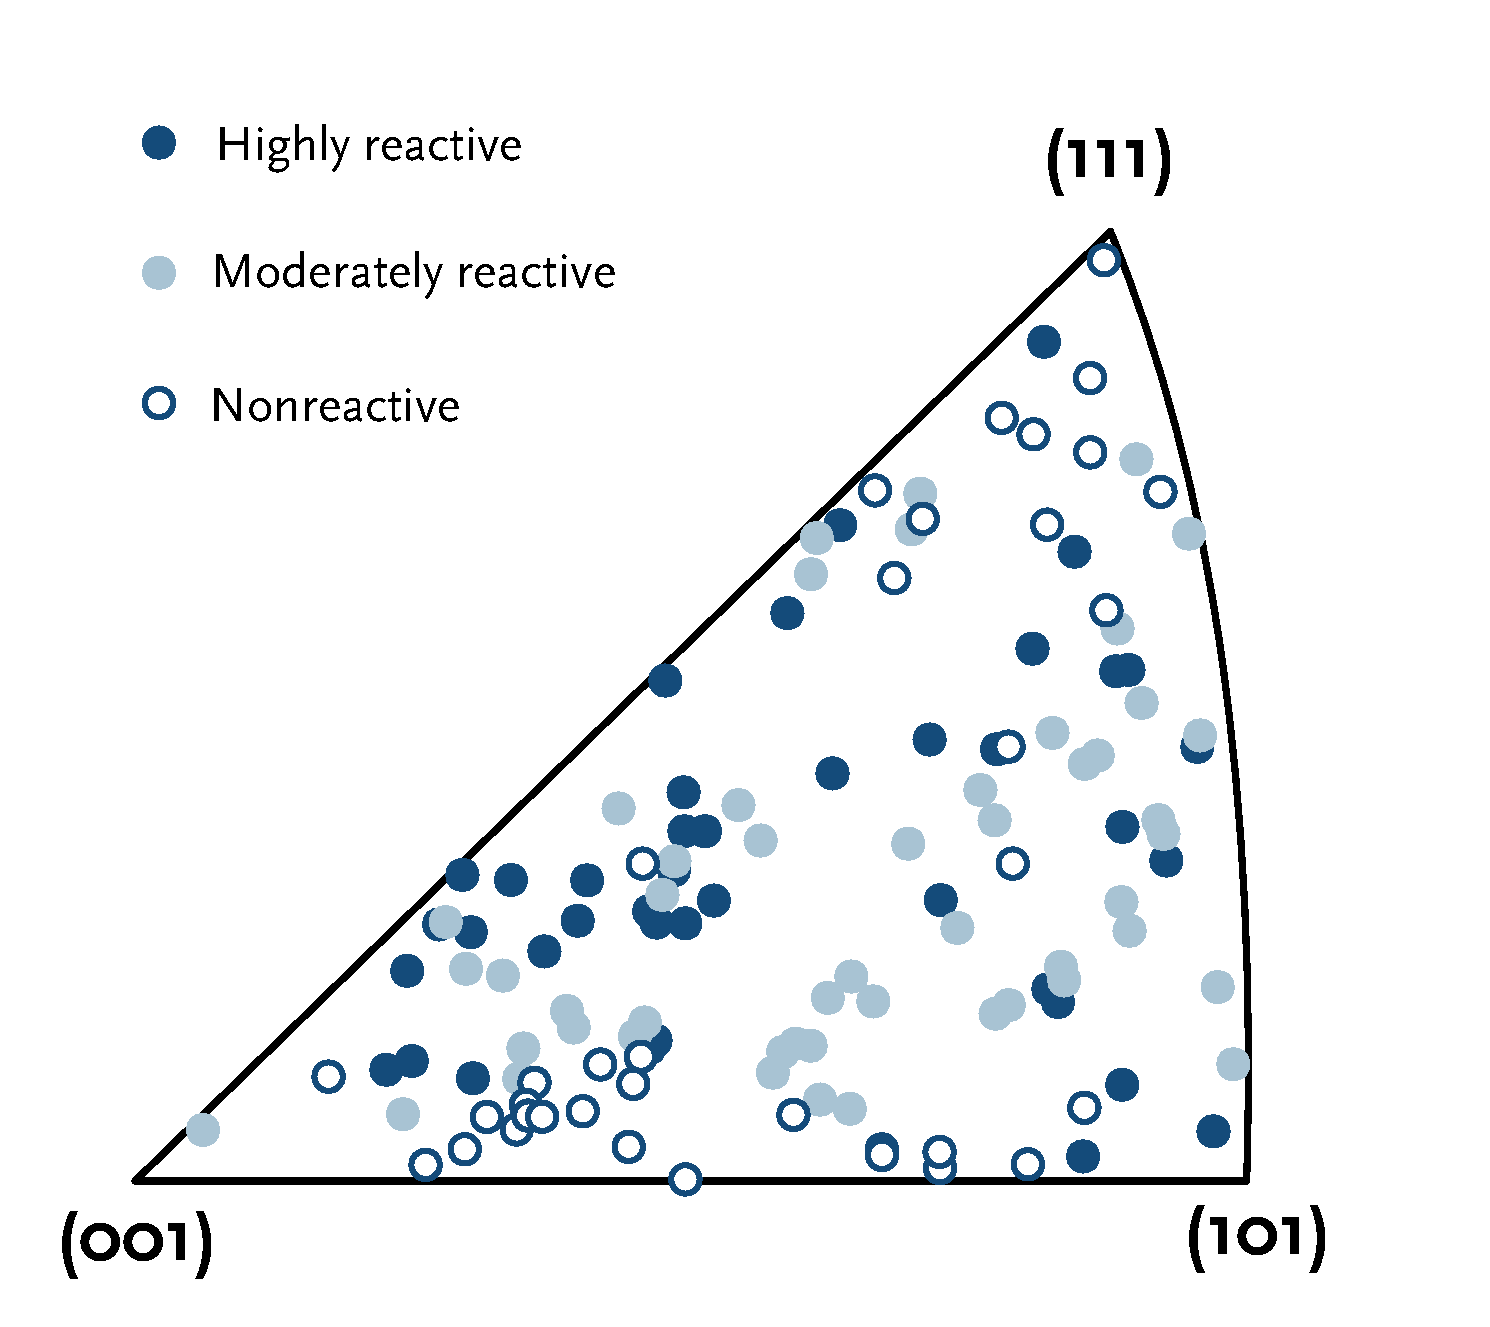
\includegraphics[width=0.6\textwidth]{substrateplot.pdf}
	\caption[Orientation of substrate grains]{%
	Standard cubic stereographic triangle showing the orientation of
	substrate grains classified in \figureref{labeledgrains}. Dark points are
	highly reactive grains, light points are moderately reactive grains,
	and empty points are nonreactive grains.}
	\label{fig:substrateplot}
	\end{center}
\end{figure}
%\sidefigure[Orientation of substrate grains]{%
%	Standard stereographic triangle showing the orientation of
%	grains classified in \figureref{labeledgrains}. Dark points are
%	highly reactive grains, light points are moderately reactive grains,
%	and empty points are nonreactive grains.
%	\label{fig:substrateplot}
%	}{%
%	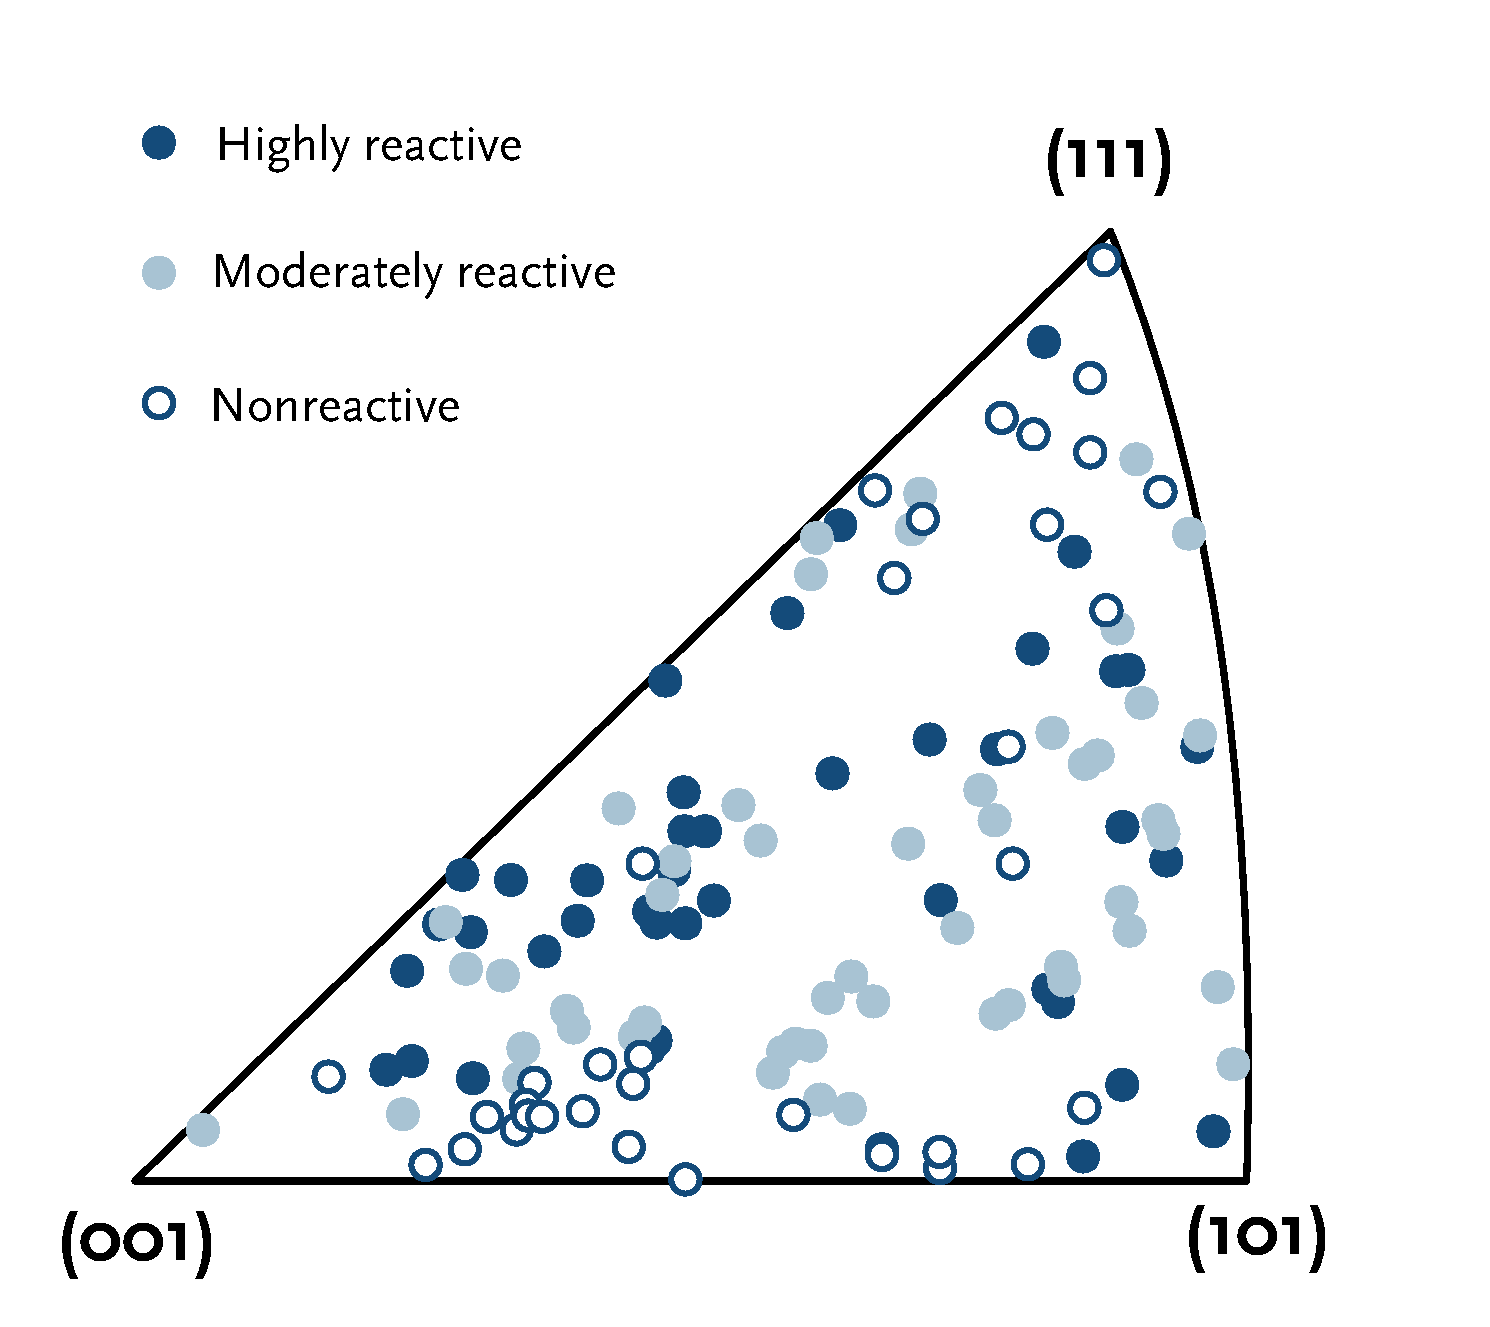
\includegraphics[width=\marginparwidth]{substrateplot.pdf}
%}{-8} % Last argument is number of lines to move up or down
In the plot of the substrate grains in \figureref{substrateplot}, highly reactive grains
are represented by dark points, moderately reactive grains by light points, and
nonreactive grains by empty points. The figure doesn't show a strong relation between
substrate orientation and grain reactivity. Highly reactive and moderately reactive points
are spread throughout the standard stereographic triangle. Nonreactive grains are weakly
clustered near the (111) orientation and along the axis between the (001) and (101)
orientations.

The reactivity of the film grains are plotted on the three hexagonal triangles in
\figureref{filmplots}. 
\begin{figure}2
	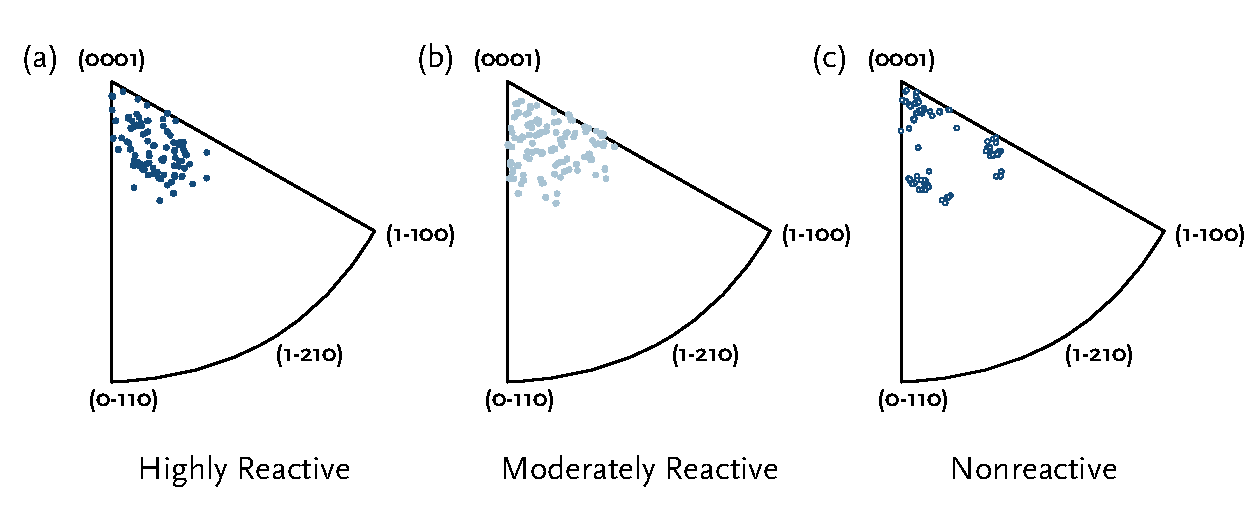
\includegraphics[width=\textwidth]{filmplots.pdf}
		\caption[Orientation of film grains]{%
			Standard stereographic triangles showing the orientation
			of (a) highly reactive (dark points), (b) moderately reactive
			(light points), and (c) nonreactive grains (empty points).}
	\label{fig:filmplots}

\end{figure}
The points are plotted in separate triangles to better illustrate trends in the data.
Because of the large number of film grains, with each substrate grain supporting multiple
film grains,\footnote{For more information on film growth, see
\chapterpageref{polycrystalline.growth}.} plotting all data on the same triangle obscures
analysis. When all points are on the same triangle, it becomes difficult to observe
individual points. The range of orientations contained in this film does not cover the
entire stereographic triangle. \figureref{filmplots} shows the entire range of
orientations for the film grains on this sample. Grains that were labeled moderately
reactive are scattered throughout the entire orientation spread. No clear orientation
preference is observed. When examining the plots for highly reactive and nonreactive
grains, the situation becomes more complicated. Highly reactive grains are clustered along
axis between the (0001) and (1\={2}13) orientations. Conversely, nonreactive grains are
clustered near the (0001) orientation and near the axis between (0001) and
(0\={1}12)/(10\={1}2) orientations. This suggests an orientation preference for
\ce{Fe2O3} films on polycrystalline \ce{SrTiO3} substrates. This is discussed further in
\sectionref{sec:poly.reac.discussion}.


\subsection{Atomic Force Microscopy}
\label{subsec:poly.reac.afm}


After optical microscopy, \abbr{AFM} was then used to confirm the interpretation of the
optical image. Five individual areas of the sample surface were scanned, each comprising
multiple substrate grains. These areas were selected to contain all reactivity classes and
a variety of substrate orientations. Representative \abbr{AFM} micrographs of the examined
areas are shown in \figureref{filmafm}.
\begin{figure}
\centering
	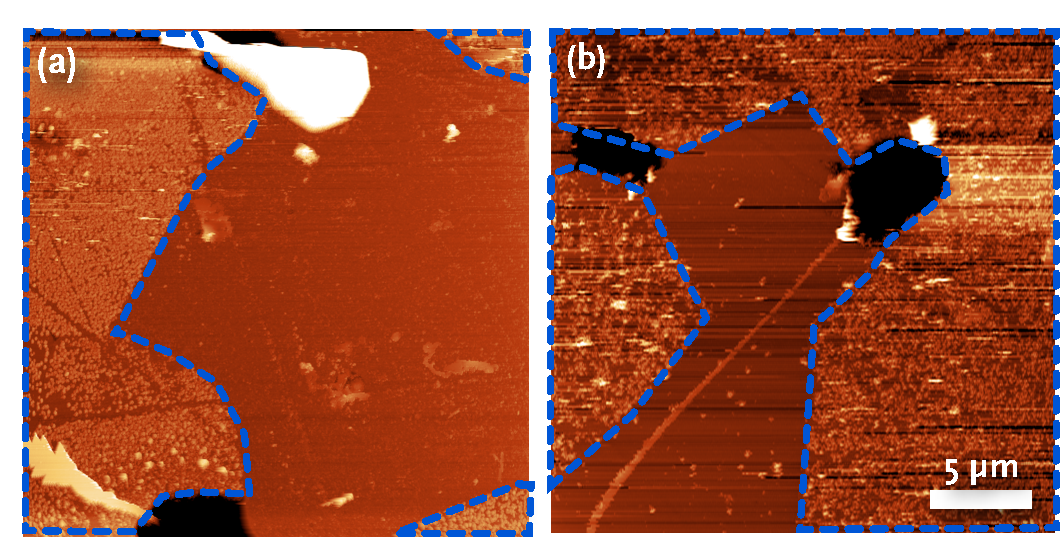
\includegraphics[width=0.8\textwidth]{filmafm.pdf}
		\caption[Representative \abbr{AFM} images of film]{%
			Representative \abbr{AFM} images of the film surface after
			reaction, showing highly reactive and nonreactive grains. The 
			areas corresponding to these micrographs are outlined in 
			Figure~\ref{fig:filmoptical}. }
	\label{fig:filmafm}
\end{figure}
Reaction product appears as bright contrast in the \abbr{AFM} images. Varying levels of
reactivity are seen in each of the micrographs. In \figureref{filmafm}(a), grains
identified as highly reactive are outlined.

The \abbr{AFM} micrographs verify the interpretation of the optical images. Grains that
were dark on the optical micrograph were the grains with the largest amount of silver
product on the surface. Grains that were bright on the optical image had the least amount
of reaction product. These results verify the broader but less detailed results from the
optical micrograph, and give increased reliability to the reactivity assignments in
\figureref{labeledgrains}. \abbr{AFM} analysis did not show a difference in roughness
between grains to account for the order of magnitude reactivity difference observed in
these results.


\section{Discussion}
\label{sec:poly.reac.discussion}


Overall, the film is more reactive than the bulk hematite. Grains with orientations that
demonstrated low reactivity in the bulk were highly reactive in the film. For similar
reaction times, the film showed more reactive grains than the bulk, as well as more
reaction product on the surface. Especially considering that the film is only
\SI{50}{\nano\meter} thick, and so is only absorbing a small portion of the incident light
before the interface with the substrate,\footnote{The penetration depth of the light in
this experiment (\textlambda = \si{470}{\nano\meter}), reported in
\sectionref{sec:single.crystal.discussion}, is \texttildelow\SI{450}{\nano\meter},
significantly larger than the thickness of the film in this experiment.} the film exhibits
high reactivity when compared to bulk \ce{Fe2O3}. Once again, the \ce{SrTiO3} substrate
improves the photochemical activity of hematite films when compared to the bulk material.

The observed trends in photochemical reactivity in this chapter represent combined effects
from \ce{Fe2O3} orientation and substrate/film interaction, each presented the previous to
chapters. In \chapterref{fe2o3orientation}, it was observed that \ce{Fe2O3} reactivity is
highly anisotropic, with c-axis oriented crystallites showing low reactivity. Conversely,
the c-axis oriented films on \ce{SrTiO3} substrates presented in
\chapterref{single.crystal.reactivity} were highly reactive. The films on polycrystalline
substrates observed here expose varying film orientations while retaining the orientation
relationship between film and substrate observed for the films in
\chapterref{single.crystal.reactivity}.\footnote{A complete description of the orientation
relationship for \ce{Fe2O3} films on polycrystalline \ce{SrTiO3} substrates can be found
in \chapterpageref{polycrystalline.growth}.}

The optical micrograph presented in \figureref{filmoptical} shows clear signs of
reactivity differences between grains. Some grains are dark, completely covered in silver
reaction product. Other grains are completely devoid of reaction product. The boundaries
between areas of high reactivity and low reactivity correlate with \abbr{EBSD} maps of the
substrate grains. Qualitatively, the \ce{Fe2O3} film on the \ce{SrTiO3} substrate is
overall significantly more reactive than the polycrystalline sample discussed in
\chapterref{fe2o3orientation}. 

The results presented in Figures \ref{fig:substrateplot} and \ref{fig:filmplots} suggest
that while the film orientation has an effect on reactivity, the substrate orientation
does not. Only the mild clustering of non reactive grains found along the axis between
(001) and (101) oriented grains suggests any direct affect of substrate orientation on
reactivity. On the other hand, the plots for highly reactive, moderately reactive, and
nonreactive films differ from each other. Highly reactive grains are clustered along the
center of the standard stereographic triangle, along the axis between (0001) and
(1\={2}10). Areas along the edge of the triangle, located at orientations between (0001)
and (10\={1}0) do have few active grains. The reverse distribution is seen for the
nonreactive grains. Nonreactive grains are clustered near the (0001) orientation, and
along the axes between (0001) and (0\={1}10)/(10\={1}0). Grains described as moderately
reactive were spread over the entire space of film orientations. 

The results here show similar trends to the anisotropic behavior of bulk hematite
crystallites.%
\footnote{%
	The discussion in this chapter is a brief overview of the results for photochemical
activity of bulk hematite polycrystals. See \chapterpageref{fe2o3orientation} for a
detailed description of the results of this experiment.
} 
It is shown in this document that bulk \ce{Fe2O3} grains located near the (1\={2}10)
orientation are the most reactive. Grains far away from this orientation exhibited
negligible reactivity. This includes (0001) (c-axis) oriented grains, and also grains at
any degree of tilt away from (0001) orientation with the [10\={1}0] direction located out
of the sample plane. 

For bulk hematite, the grains that were the most reactive were located relatively near to
to the (1\={2}10) orientation. The reactive grains in \figureref{filmplots}(a) are tilted
considerably closer to (0001) than any of the reactive grains in that study. However, the
results here do follow the general trend observed for that work; hematite grains become
reactive as they tilt away from the (0001) orientation, \emph{so long as the [1\={2}10]
direction is pointing out of the surface}. In other words, if the axis of rotation away
from (0001) is a [10\={1}0] direction, the [1\={2}10] direction will be pointing out of
the surface, and the grain is likely to be reactive.\footnote{\figurepageref{fe2o3axes}
provides a helpful schematic of the relative orientation of the [10\={1}0] and [1\={2}10]
directions and planes in the hematite crystal system.} If the tilt axis is the [1\={2}10]
direction, the grain is not likely to be reactive, as the orientation will lie along the
nonreactive region between (0001) and (10\={1}0). The results for the film materials show
the same trend, however the film becomes reactive and a much lower tilt away from (0001).
Compare the distribution of reactive grains in \figureref{filmplots} to the distribution
in Figures \ref{fig:semtriangle} or \ref{fig:afmtriangle} in
\chapterref{fe2o3orientation}. It is important to note that the higher symmetry of the
cubic substrate limits the range of possible orientations for the hexagonal film.
The most highly reactive bulk orientations are not present in this film, and yet
many film grains are highly reactive.

For the films on single crystal substrates in \chapterref{single.crystal.reactivity},
(0001)-oriented films on (111)-oriented substrates were highly reactive. Here, many grains
close to this substrate orientation were marked as nonreactive or moderately reactive. The
contradictory results can be understood through the anisotropic reactivity of hematite.
For all \ce{Fe2O3} films on \ce{SrTiO3} substrates, the reactivity of the film was
improved compared to the bulk material. When grown on single crystal substrates, the only
film orientation observed is (0001)  basal plane oriented \ce{Fe2O3}. This orientation is
nonreactive for bulk crystals. When films are grown on polycrystalline substrates, more
reactive \ce{Fe2O3} orientations are exposed to the surface. If single crystal substrates
existed that could be used to stabilize the reactive faces of \ce{Fe2O3}, it is expected
that those films would be even more reactive than the films in the previous chapter.
However, the low-index orientations available for \ce{SrTiO3} substrates do not stabilize
such films. The results in this chapter suggest that the anisotropic reactivity of
\ce{Fe2O3} persists, but is less severe as a result of substrate/film interactions.

An interesting phenomenon observed for this experiment is that reactivity in some cases
appears to be different between film grains on the same substrate. One set of grains is
sometimes more reactive than the other. Reactivity following the lamellar structure of the
film grains is observed in multiple instances in \figureref{filmoptical}. These cases were
generally those of moderate reactivity, and all film grains on that substrate grain were
plotted as mildly reactive in \figureref{filmplots}. It may be that further refinement in
the orientation depends of hematite reactivity could be observed through an analysis of
these grains. However the detail of the optical image was not sufficient to accurately
determine which grains followed this reactivity pattern. Additionally,
\figureref{labeledgrains} suggests that grains with similar levels of
reactivity are clustered near each other. The highly reactive grains are all located near
each other, as are many of the nonreactive grains. This could suggest that the high
reactivity on some parts of the sample is not directly related to individual crystallite
orientation. However, the boundaries between highly active grains and nonreactive grains
do sharply follow the grain boundaries identified using \abbr{EBSD}. The results presented
in this document do not entirely support the assertion that another affect could be 
responsible for the high reactivity and resulting clustering of reactive grains. However, 
the clear demarcation in reactivity across grain boundaries suggest that there is some 
effect related to individual crystallite properties.
 



\section{Conclusions}
\label{sec:poly.reac.conclusions}

Hematite films on polycrystalline substrates showed clear signs of reactivity differences
between grains. Substrate orientation does not appear to drive this reactivity difference,
except in that it also is responsible for resulting film orientation. The film orientation
shows a correlation between orientation and high and low reactivity. Highly reactive
grains were found in the region between (0001) and (1\={2}13) on the standard
stereographic triangle. Nonreactive grains were clustered near (0001) and in the region
between (0001) and (10\={1}2)/(01\={1}2). This pattern is similar to the orientation
dependent reactivity observed in \chapterref{fe2o3orientation}. Additionally, the film on
average was significantly more reactive than bulk hematite. 
